\documentclass{beamer}

\mode<presentation> {
\usetheme{Copenhagen} % Pretty neat, soft color.
\setbeamercovered{transparent}
\setbeamercovered{invisible}
\setbeamertemplate{navigation symbols}{} 
}

\usepackage{graphicx,amssymb}
\usepackage{amsmath}
\usepackage{bm} 
\usepackage{wasysym}

\title[ECML/PKDD 2011 demo session (demo \#10)]{InFeRno - an Intelligent Framework for Recognizing Pornographic Web pages}
\author{\bf{\underline{S. Karavarsamis}, N. Ntarmos and K. Blekas }}

\institute[UoI]
{\large
Department of Computer Science\\
University of Ioannina, Ioannina, Greece \\
\medskip
{\normalsize E-mail: \{cs061205, ntarmos, kblekas\}@cs.uoi.gr}
}
\date{}

\begin{document}

\begin{frame}
\titlepage
\end{frame}

\begin{frame}
\frametitle{Problem preliminaries and intuition}

\begin{itemize}

	\item Motivation:
	\begin{enumerate}
		\item Lots of "bad" pages out there
		\item Human-driven classification is highly impractical
		\item Need for an unobtrusive filtering method
	\end{enumerate}

	\item Main characteristics of our system:
	\begin{enumerate}
		\item A minimal but powerful vector space
		\item An extra "bikini" class
		\item A highly accurate and fast classification scheme
		\item An implementation of the classifier as a standalone
		network service (ubiquity and ease of use)
		\item Integreation of the classifier with off-the-shelf web proxy cache server through an ICAP interface (can be transparently applied to whole networks)
	\end{enumerate}
\end{itemize}

\end{frame}

\begin{frame}
\frametitle{InFeRno architecture}
\begin{center}
	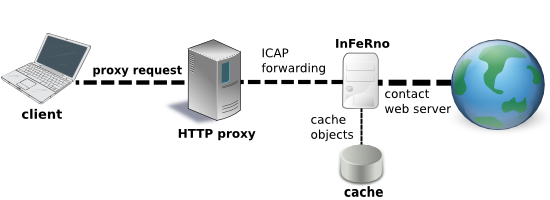
\includegraphics[scale=0.6]{images/network_diagram.png}
	\begin{enumerate}
		\item Implementation of the InFeRno core as an ICAP module (integrates well with most HTTP proxy servers)
		\item Decoupled image classification and web page preprocessing (network I/O, image-score fusion)
		\item Using a fast ISAM-based cache for fast  I/O (classification lookups, updates, etc)
        \item Flexible configuration (multiple classification + network parameters)
	\end{enumerate}
\end{center}
\end{frame}

\begin{frame}
\frametitle{Classification System}
\begin{center}
		\begin{tabular}[c]{cccc}
			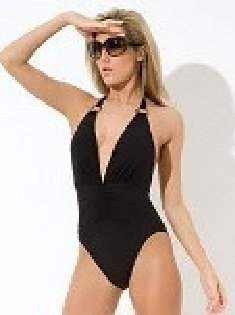
\includegraphics[width=.10\columnwidth]{images/orig.pdf}  \ &
			
\includegraphics[width=.10\columnwidth]{images/skin.pdf} \ &
			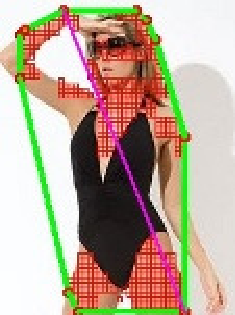
\includegraphics[width=.10\columnwidth]{images/grid.pdf} \ &
			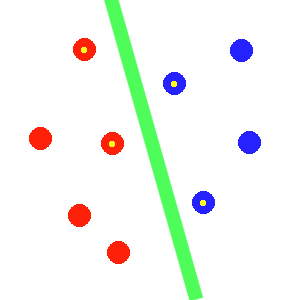
\includegraphics[width=.10\columnwidth]{images/svm.png} \ \\
			\normalsize{original} & \normalsize{skin} & \normalsize{contour} & \normalsize{SVM}\\
			\normalsize{image} & \normalsize{detection} & \normalsize{extraction} & \normalsize \\
		\end{tabular}
\end{center}

{\underline {\bf Three stages}}
     \begin{enumerate}
        \item Skin detection (rule-based)
        \item Contour extraction (region splitting scheme)
		\item Feature extraction and Classifier
		  \begin{itemize}
			\item Extracted 15 features: RGB color statistics, skin-to-nonskin ratio, contour orientation, Hu moments
	        \item SVM classifier with RBF kernel
	       \end{itemize}
	\end{enumerate}

\end{frame}

\begin{frame}
\frametitle{Experimental results}
	\begin{itemize}

		\item Training dataset: manually collected 680 bikini images, 
		      660 porn images and 4260 benign images from the Web

		\item Comparison with the EU-funded {\em POESIA pornography elimination system}

		\item Results:
	          \begin{center}
		             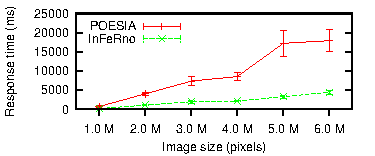
\includegraphics[scale=1.3]{images/scatter-p-t-all-bars.pdf}
	          \end{center}
			  \begin{itemize}
	                \item \textbf{4x speedup} improvement 
                    \item High accuracy (comparable to POESIA for images and image-only pages)
	          \end{itemize}
	\end{itemize}
\end{frame}

\begin{frame}
	\centerline{Thank you for your attention! \smiley}
\end{frame}

\end{document} 
